\section[Contributing to the Question Pool]{Contributing}

\begin{frame}
  \frametitle{Contributions via the HPCCF-Wiki}
  \centering
  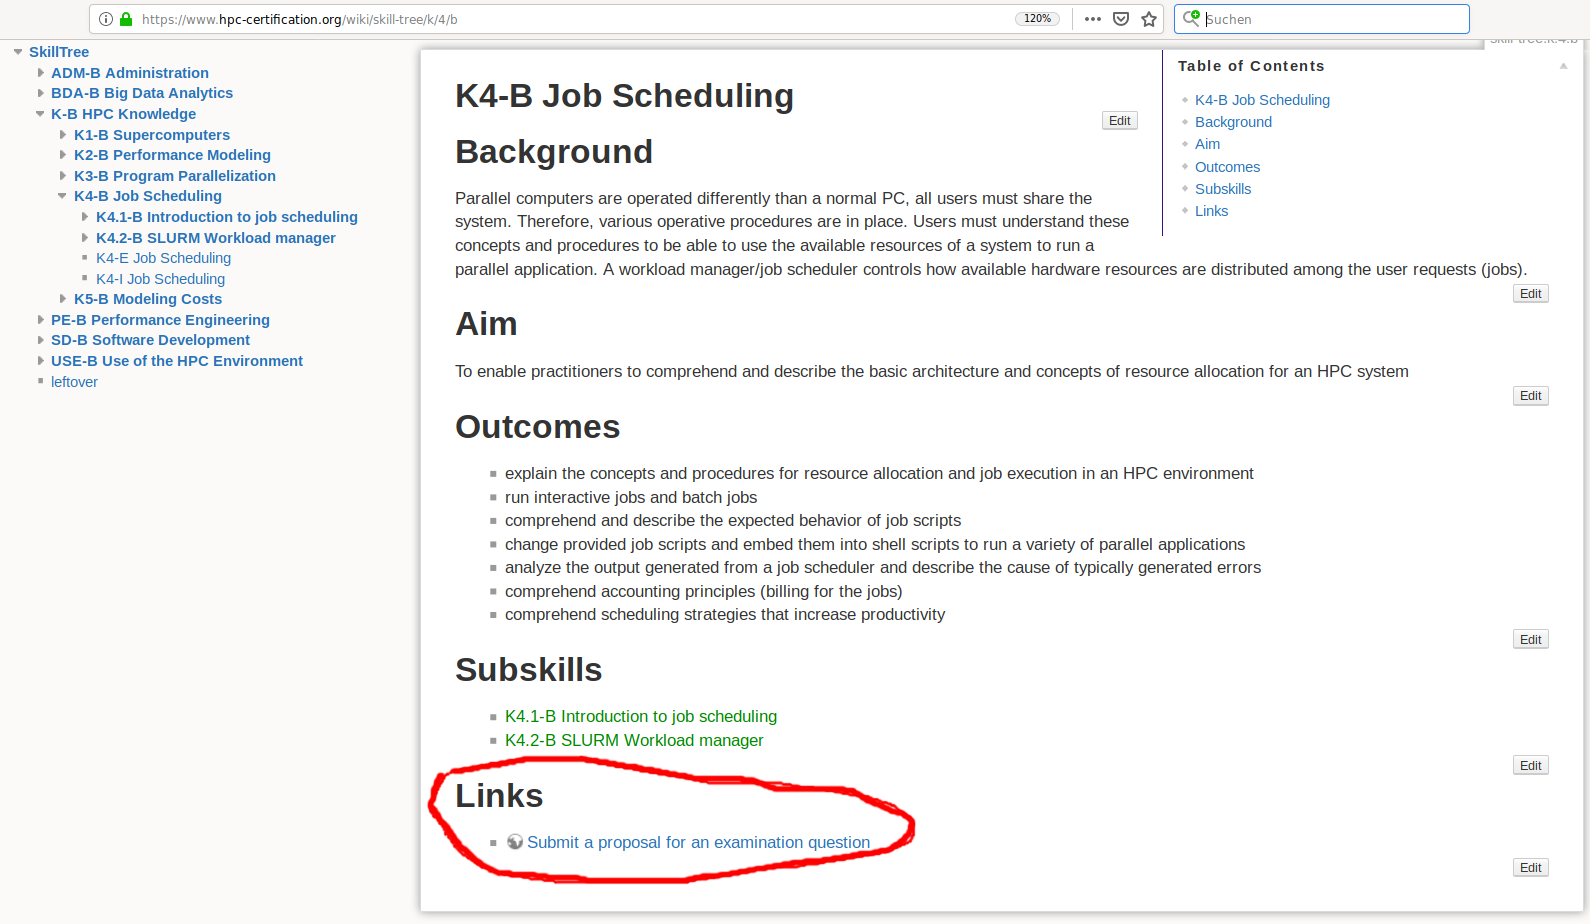
\includegraphics[width=0.8\textwidth]{images/contribution}
\end{frame}


\begin{frame}
  \frametitle{Contributions via the HPCCF-Wiki II}
  Each \lhref{https://www.hpc-certification.org/wiki}{HPCCF wiki} page contains a link. It leads to a little form asking for:
  \begin{itemize}
   \item contact mail
   \item to select a learning objective from a pre-formatted list
   \item to supply the question you thought of
   \item and (in case of a multiple choice question) the possible answers.
  \end{itemize}
  \pause
  \task[Evaluation Process]{Now, HPCCF-member evaluate the submitted question. If approved, it will be formatted and merged into the pool of questions for the choosen topic / skillset.}
\end{frame}

